Como complemento a la lectura de este capítulo se recomienda tener una copia
local del repositorio del proyecto, disponible para su libre descarga desde la
forja oficial~\cite{forja}.

\section{Entorno de construcción}

En esta sección se detalla el marco tecnológico utilizado para la construcción
del sistema, basándonos en lo presentado en la
sección~\ref{sec:alternativas-solucion},\textit{~\nameref{sec:alternativas-solucion}}.

\subsection{Aplicación web}

El entorno tecnológico de la aplicación web ha resultado ser muy variado y rico
en tecnologías en total vigencia en la actualidad. 

\subsubsection{Herramientas de diseño y desarrollo}

Como editor principal se ha utilizado \textbf{Sublime Text
  2}~\cite{sublime-text}, un editor freeware escrito en Python especialmente
dotado para el desarrollo de aplicaciones web. Cuenta con un gran número de
características que lo han hecho destacar en los últimos años, como la habilidad
de seleccionar y editar a la vez varios fragmentos de texto, el rápido motor de
\textit{búsqueda difusa} para encontrar ficheros y cadenas o su capacidad de
extensión a través de paquetes escritos por terceros y fácilmente instalables.

Para ciertas tareas, como la escritura de la presente memoria, se ha hecho uso
del veterano editor \textbf{Emacs}~\cite{emacs}, que sigue siendo la mejor
opción a la hora de editar documentos de \LaTeX. 

Se ha utilizado \textbf{draw.io}~\cite{draw.io} para la generación de diagramas
de casos de uso, secuencia, diagramas de flujo y similares. Se trata de una
herramienta web, actualmente integrable en Google Drive, con un enorme número de
elementos de dibujo y la capacidad de exportar en un gran número de formatos,
entre ellos en formato vectorial \ac{PDF}. Para el diseño visual de las
interfaces de usuario se ha utilizado \textbf{Adobe Photoshop}~\cite{photoshop}.

\subsubsection{Gestión de dependencias}
\label{subsec:gestion-dependencias}

Para facilitar la gestión de las dependencias del proyecto se han utilizado
\textbf{VirtualEnv}~\cite{virtualenv} y
\textbf{VirtualEnvWrapper}~\cite{virtualenvwrapper}. Estas herramientas permiten
generar \textit{entornos virtuales} para cada proyecto, en los que se instalan
las dependencias necesarias. Estos entornos se activan y desactivan, de forma
que las bibliotecas instaladas en el entorno virtual de un proyecto no son
accesibles desde el entorno del otro proyecto. Esto evita la polución del nivel
general de bibliotecas y facilita el control estricto de las versiones de las
dependencias. 

Junto a virtualenv, la herramienta \textbf{pip}~\cite{pip} permite guardar en un
fichero anexo la lista de dependencias de un proyecto, de forma que sea fácil
reinstalarlas todas si hubiese que repetir la instalación en otro sistema.

\subsubsection{Control de versiones}

Todo el código fuente del proyecto se encuentra alojado en un repositorio
público en \textbf{GitHub}~\cite{forja}, haciendo uso de los planes
gratuitos. GitHub es una forja que utiliza el sistema de control de versiones
\textbf{Git}~\cite{git}. Además del alojamiento de código, GitHub provee
numerosas funcionalidades adicionales, tanto a nivel social (permitiendo a las
forjas tener \textit{followers}, por ejemplo) como a nivel funcional (ofreciendo
sistemas de tickets, estadísticas, etcétera).

El uso de un control de versiones es fundamental por varios motivos. En primer
lugar, sirve como sistema de copia de seguridad. En segundo lugar, permite
deshacer cambios en el código que no funcionen bien, siendo siempre posible
\textit{volver atrás}. Por último, sirve como \textit{cuaderno de bitácora}
improvisado, ya que se guarda el historial de \textit{commits} que el
desarrollador va enviando junto a los mensajes, siendo posible ver en una línea
temporal el progreso del trabajo.

\subsubsection{Lenguaje de programación}

Como se ha comentado en numerosas ocasiones en la presente memoria, el lenguaje
de programación elegido para el desarrollo del proyecto es
\textbf{Python}~\cite{Python}, un lenguaje interpretado de alto nivel
desarrollado por Guido Van Rossum en 1991. Python soporta múltiples paradigmas
de programación, desde la orientación a objetos hasta la programación funcional,
pasando por el clásico estilo imperativo. Su principal uso ha sido como lenguaje
de scripting, pero también tiene su hueco en contextos más amplios como lenguaje
principal.

Su facilidad de aprendizaje, lo simple de su sintaxis (basada en la indentación
para marcar los bloques) y su extensibilidad (sobre todo gracias al uso de
métodos \textit{mágicos} y metaprogramación) han hecho que el lenguaje sea muy
popular y su uso en los últimos años se haya expandido enormemente.

\subsubsection{Framework de desarrollo}

El framework de desarrollo elegido es \textbf{Django}~\cite{django}, un
proyecto de código abierto nacido en 2005. La meta fundamental de Django es
facilitar la creación de sitios web complejos, haciendo especial hincapié en
mantener un ritmo de desarrollo rápido y evitar la duplicidad de código. Así,
gran parte del potencial de Django es la gran cantidad de funcionalidad que ya
trae integrada, ya sea en el propio núcleo del framework o a través de
\textit{apps} oficiales que se incluyen en la distribución oficial.

Los elementos más destacables de Django son:

\begin{itemize}
\item Un sistema de mapeo objeto-relacional, que facilita enormemente el trabajo
  con elementos de bases de datos a través de instancias de modelos.
\item Un sistema de procesamiento de peticiones a través de vistas.
\item Un despachador de URLs basado en expresiones regulares.
\item Soporte para plantillas.
\item Un sistema de autenticación extensible.
\item Una interfaz de administración que se adapta dinámicamente a cualquier proyecto.
\item Un sistema de comentarios.
\item Soporte integrado contra numerosos tipos de ataques vía web, como
  inyección SQL o cross-site scripting.
\end{itemize}

\subsubsection{Nivel de persistencia}

\textbf{SQLite} es un sistema de gestión de bases de datos relacional de dominio público,
contenido en una pequeña biblioteca. A diferencia de los sistema de gestión de
bases de datos cliente-servidor, el motor de SQLite no es un proceso
independiente con el que el programa principal se comunica. En lugar de eso, la
biblioteca SQLite se enlaza con el programa pasando a ser parte integral del
mismo. El programa utiliza la funcionalidad de SQLite a través de llamadas
simples a subrutinas y funciones. Esto reduce la latencia en el acceso a la base
de datos, debido a que las llamadas a funciones son más eficientes que la
comunicación entre procesos. 

El conjunto de la base de datos (definiciones, tablas, índices, y los propios
datos), son guardados como un sólo fichero estándar en la máquina host. Este
diseño simple se logra bloqueando todo el fichero de base de datos al principio
de cada transacción. Esto no impide que varios procesos o hilos pueden acceder a
la misma base de datos sin problemas.

En general, SQLite no suele ser la mejor opción en sistemas de producción muy
extensos, pero para proyectos de menor envergadura su rendimiento es más que
suficiente.

\subsubsection{Gestión de tareas}

Para la gestión de tareas de forma asíncrona se ha utilizado \textbf{Celery},
una cola de tareas asíncrona enfocada a operaciones en tiempo real. Celery está
escrito en Python, pero se integra fácilmente con cualquier otro sistema que
implemente su interfaz. Las unidades de ejecución básicas, las \textit{tareas},
se ejecutan de forma concurrente en uno o varios \textit{workers}. Las tareas
pueden ejecutarse de forma asíncrona, en segundo plano, o de forma síncrona,
haciendo que el flujo de ejecución espere hasta que el resultado de la tarea
esté disponible.

Celery se comunica mediante mensajes, normalmente utilizando un \textbf{broker}
que media entre los clientes y los workers. Para iniciar una tarea, el cliente
pone un mensaje en la cola del broker. Entonces, el broker entrega el mensaje al
worker de Celery. La opción recomendada, y la que se ha utilizado en SiteUp, es
usar \textbf{RabbitMQ} como broker de mensajes.

RabbitMQ, y la mayoría de brókers de mensajes, implementan el protocolo
\ac{AMQP}, un estándar abierto para enviar mensajes entre aplicaciones y
organizaciones, siempre que éstas sean capaces de interactuar usando las
interfaces del protocolo.

\subsubsection{Herramientas de frontend}

Para el desarrollo del frontend de la web, esto es, lo que el usuario acaba
viendo y utilizando en el navegador, se han utilizado varias tecnologías,
herramientas y bibliotecas.

En primer lugar, la base de la web está escrita en \textbf{HTML5}~\cite{html5},
un lenguaje de marcado usado para estructurar y presentar contenido en la
web. Es la quinta revisión del estándar \ac{HTML}, y su objetivo principal es
unificar la sintaxis tan dispersa que había generado el uso de HTML4 y
XHTML. Además, introduce una serie de elementos (etiquetas) con contenido
semántico, tales como \texttt{<section>} y \texttt{<article>}. En la actualidad
la especificación de HTML5 no está cerrada y siguen añadiéndose cambios. Es por
ello que la compatibilidad con los navegadores no es total, aunque sí muy
extensa.

Una buena práctica en el desarrollo web es desacoplar lo máximo posible el
contenido de un documento (definido con HTML) del diseño del mismo, que
habitualmente se define usando \textbf{\ac{CSS}}~\cite{css}. En particular, en
SiteUp se ha utilizado CSS3, la última versión del estándar. CSS permite la
definición de \textbf{estilos} que se aplican a \textbf{elementos} de una web,
mediante \textbf{reglas}. Así, las reglas se componen de un selector, que define
los elementos a los que se le aplicará el estilo, y un bloque de declaración, en
el que se describen las propiedades que se le aplicarán al elemento. Hay un gran
número de reglas para la definición de selectores, y una extensa lista de
propiedades definibles en CSS.

A pesar de todo, CSS cuenta con una serie de limitaciones de base. Por ejemplo,
no cuenta con mecanismos sencillos para favorecer la modularidad del código. Por
ello han surgido una serie de \textit{metalenguajes} que añaden nuevas
características para facilitar el desarrollo pero que, al final, acaban
generando código CSS compatible. Uno de estos metalenguajes es
\textbf{\ac{Sass}}~\cite{sass}. Entre las funcionalidades que Sass añade se
encuentran:

\begin{itemize}
\item Definición de variables.
\item Anidamiento de reglas.
\item Uso de \textit{mixins}.
\item Herencia de selectores.
\end{itemize}

Además, Sass cuenta con bibliotecas de terceros, como
\textbf{Compass}~\cite{compass}, un framework de desarrollo que añade a Sass
numerosas utilidades adicionales.

Con HTML5 y CSS3 es posible crear perfectamente sitios web con animaciones y
funcionalidad básica, pero en SiteUp era necesario tener cierta interactividad a
la hora de, por ejemplo, mostrar gráficas. Para ello resulta necesario utilizar
un lenguaje de scripting para web, y ese lenguaje es
\textbf{JavaScript}~\cite{javascript}. Se trata de un lenguaje dinámico
utilizado principalmente para añdir dinamismo a los sitios web. Se lanzó en 1995
y desde entonces ha ido mejorando con el tiempo, sobre todo con la adición de
numerosas \ac{API} en los navegadores. El problema que ha tenido JavaScript es
el irregular soporte de los diferentes navegadores, sobre todo las versiones de
Internet Explorer. Así, era habitual utilizar código distinto para realizar el
mismo procedimiento según fuese el navegador.

Afortunadamente existen bibliotecas de desarrollo que actúan como capa de
abstracción y permiten al desarrollador olvidarse de las diferencias de
compatibilidad entre navegaores. La biblioteca más conocida para uso general es
\textbf{jQuery}~\cite{jquery}. Creada en 2006 por John Resig, se estima que más
del 50\% de \textbf{todos} los sitios web a nivel mundial usan jQuery. Su
popularidad se debe sobre todo a su facilidad de uso, su ligereza y la potencia
que ofrece. Por suerte la evolución de los navegadores está permitiendo
que el soporte nativo de JavaScript sea cada vez mejor, siendo progresivamente
menos necesario el uso de bibliotecas \textit{unificadoras} como jQuery, aunque
su utilidad a la hora de trabajar, por ejemplo, con efectos o con cargas
asíncronas de datos (\ac{AJAX}) sigue siendo vigente.

Para el renderizado y muestra de las gráficas, en SiteUp se ha usado
\textbf{D3.js}~\cite{d3}, una bibilioteca para la manipulación de documentos
basada en datos. D3 permite generar interesantes visualizaciones de multitud de
tipos, teniendo además capacidad para añadir interactividad, animaciones y
propiedades dinámicas. Las gráficas generadas por D3 normalmente utilizan
\ac{SVG}, por lo que el rendimiento es muy alto.


\subsubsection{Bibliotecas de terceros para backend}

En el proyecto se han utilizado un gran número de bibliotecas auxiliares para
facilitar el desarrollo y ampliar la funcionalidad de forma sencilla.

\paragraph{South}

South~\cite{south} es una biblioteca para Django que permite generar
\textbf{migraciones} de datos y estructurales de la base de datos. El término
\textit{migración} hace referencia a una modificación estructural en la que se
definen de forma lógica las diferencias entre el estado anterior y el posterior,
de forma que sea posible trasladar o \textit{transformar} los datos de un estado
a otro, incluso dando la posibilidad de deshacer los cambios. 

Es una función de gran utilidad, y muchos otros frameworks, como \textit{Ruby on
  Rails}, incorporan este mecanismo de forma nativa. South se ha hecho tan
popular y común que su código ha sido integrado en Django de forma nativa a
partir de la versión 1.7.

\paragraph{Fabric}

Fabric~\cite{fabric} se compone de una herramienta de línea de comandos y una
biblioteca que facilitan la comunicación con servidores remotos a través de
SSH, facilitando el despliegue de aplicaciones y las tareas de administración.

Provee un conjunto básico de operaciones para ejecutar, ya sea forma local o
remota, operaciones de toda clase: desde comandos de shell hasta subida y
descarga de ficheros, pasando por funciones auxiliares.

En SiteUp, Fabric se ha utilizado para facilitar el despliegue de la plataforma
web en el servidor remoto. Para ello, se desarrolló un fichero
\texttt{fabfile.py}, que se encuentra en la raíz del proyecto web, que define
las operaciones a realizar. Cuando se ejecuta el siguiente comando:

\begin{bashcode}
$ fab deploy  
\end{bashcode}

El sistema realiza las siguientes operaciones en el servidor remoto:

\begin{itemize}
\item Activa el entorno virtual (\textit{virtualenv}).
\item Descarga los últimos cambios del código desde la forja~\cite{forja}.
\item Instala los nuevos requisitos definidos mediante el fichero de requisitos
  del entorno virtual (véase la sección \ref{subsec:gestion-dependencias}
  \textit{\nameref{subsec:gestion-dependencias}}).
\item Dispone los ficheros estáticos del proyecto en un directorio especial,
  para que el servidor web pueda servirlos (véase la sección
  \ref{subsec:arquitectura-logica-web}, \textit{\nameref{subsec:arquitectura-logica-web}}).
\item Aplica cualquier cambio que se haya realizado a la estructura de la web
  mediante migraciones.
\item Reinicia los servicios.
\end{itemize}

La reducción de tiempo es considerable y la facilidad de uso es total.

\paragraph{django-braces}

Se trata de una extensión de Django que provee un conjunto de \textit{mixins}
que agregan funcionalidad a las vistas de forma sencilla. 

Un \textbf{mixin} es una clase que ofrece cierta funcionalidad para ser
hererdada por una subclase, pero que no está pensada para funcionar por sí misma
de forma autónoma. Así, la herencia que se produce al heredar de un mixin es
básicamente un mecanismo para integrar funcionalidad adicional, en lugar de una
herencia en el sentido clásico. 

Entre la funcionalidad que provee \texttt{django-braces} se encuentran, por
ejemplo, mixins para controlar el acceso a zonas para usuarios registrados o
para devolver fácilmente respuestas JSON.

\paragraph{django-extensions}

Se trata de una colección de extensiones para Django de muy diversos tipos:
ccomandos de administración, extensiones para la zona de administración,
etcétera.

Algunas de las utilidades más interesantes que provee son las siguientes:

\begin{itemize}
\item El comando \texttt{shell\_plus} provee una shell que carga automáticamente
  todos los modelos de la aplicación, de forma que sea fácil hacer consultas
  rápidas a la base de datos.
\item El comando \texttt{graph\_models} genera automáticamente un diagrama
  visual con el modelo Entidad-Relación de la base de datos.
\end{itemize}

\paragraph{django-debug-toolbar}

Proporciona una barra con extensa información de depuración: tiempos de cpu y
renderizado, consultas SQL ejecutadas, plantillas utilizadas, variables de
entorno y de petición, ficheros estáticos, señales dadas de alta, mensajes de
registro...

Esta extensión es uno de los mecanismos de depuración más utilizados en los
proyectos Django de todo el mundo. Además, automáticamente se desactiva en
entornos de producción, por lo que no supone un problema.

\subsection{Aplicación móvil}

El entorno tecnológico de la aplicación móvil es el estándar para el desarrollo
de aplicaciones Android hoy en día, que consta de los siguientes elementos.

\subsection{Herramientas de desarrollo}

Para el desarrollo de la aplicación móvil se ha optado por utilizar
\textbf{Android Studio}~\cite{android-studio}, un entorno de desarrollo
integrado basado en el popular software IntelliJ IDEA y perfectamente
personalizado con las bibliotecas y herramientas necesarias para el desarrollo
de aplicaciones Android.

Está preparado y gestionado por Google, y aunque está en una etapa temprana de
desarrollo, su uso es totalmente viable y los resultados son correctos. Incluye
elementos muy útiles, como la integración con los servicios de \textbf{Google
  Cloud Messaging}, que se han utilizado en el proyecto (véase la
sección~\ref{subsec:arquitectura-logica-android},
\textit{\nameref{subsec:arquitectura-logica-android}}).


\subsection{Servicio de notificaciones}

Para el envío y la recepción de notificaciones se ha utilizado el servicio
\textbf{Google Cloud Messaging for Android}. Se trata de un servicio gratuito
que permite enviar datos desde un servidor a dispositivos Android que
previamente se hayan registrado a través de una aplicación en particular.

El flujo de funcionamiento es el siguiente:
\begin{enumerate}
\item El usuario instala la aplicación, por ejemplo \textit{SiteUp Client}.
\item La aplicación conecta con los servidores de GCM y pide el \textbf{código
    de registro} del dispositivo, que lo identifica unequívocamente.
\item La aplicación guarda ese código en el servidor de la plataforma web.
\item En caso de necesitar enviar una notificación, la plataforma web hace una
  petición al servidor de GCM, enviando el código de registro del dispositivo al
  que enviar la notificación y, lógicamente, el contenido de la notificación.
\item El servidor de GCM se encarga de transmitir la notificación al dispositivo
  Android.
\item El dispositivo recibe la notificación, siendo la aplicación móvil la
  encargada de actuar en consecuencia, mostrando un mensaje o realizando
  cualquier otra operación.
\end{enumerate}

La facilidad con la que se pueden enviar mensajes de esta manera, de forma
instantánea, es asombrosa y pone de manifiesto las facilidades que la plataforma
Android pone a los desarrolladores.

\section{Organización del código fuente}

En esta sección se detalla la organización del código fuente del proyecto,
describiendo la utilidad de los ficheros y directorios.

El código fuente presente en la forja~\cite{forja} cuenta con los siguientes
elementos en el directorio raíz:

\begin{itemize}
\item \texttt{android-client}: código fuente de la aplicación Android.
\item \texttt{logs}: directorio con los ficheros de registro.
\item \texttt{memoria}: directorio con el código fuente de la presente memoria.
\item \texttt{web}: código fuente de la plataforma web.
\item \texttt{LICENSE}: fichero con el texto de la licencia.
\item \texttt{INSTALLING-web.md}: fichero con instrucciones de instalación de la plataforma web.
\item \texttt{README.md}: fichero de presentación para la forja.
\end{itemize}

\subsection{Plataforma web}

El código de la plataforma web se encuentra íntegramente contenido en el
directorio \texttt{web} del proyecto, que contiene lo siguiente:

\begin{itemize}
\item \texttt{db}: directorio donde se guarda la base de datos y otros ficheros.
  \begin{itemize}
  \item \texttt{celerybeat.db}: datos del servicio Beat de Celery.
  \item \texttt{django-db.sqlite3}: base de datos principal SQLite.
  \end{itemize}
\item \texttt{siteup}: directorio con ficheros a nivel de proyecto.
  \begin{itemize}
  \item \texttt{settings}: directorio de configuraciones.
    \begin{itemize}
    \item \texttt{base.py}: configuración general.
    \item \texttt{local.py}: configuración para entorno local de desarrollo.
    \item \texttt{production.py}: configuración para entorno de producción
    \end{itemize}
  \item \texttt{celery.py}: configuración de Celery.
  \item \texttt{urls.py}: configuración de rutas de acceso web y URLs.
  \item \texttt{wsgi.py}: configuración del punto de acceso para el servidor WSGI.
  \end{itemize}
\item \texttt{siteup\_api}: directorio de la app que gestiona la API.
  \begin{itemize}
  \item \texttt{migrations}: directorio de migraciones generadas por South.
  \item \texttt{tests}: directorio con los tests de la aplicación.
  \item \texttt{admin.py}: configuración de la app para el panel de administración.
  \item \texttt{managers.py}: gestores de modelos personalizados.
  \item \texttt{models.py}: definiciones de los modelos de la base de datos.
  \item \texttt{utils.py}: funciones auxiliares.
  \item \texttt{validators.py}: validadores personalizados para formularios y
    campos de modelos.
  \item \texttt{views.py}: vistas de acceso.
  \end{itemize}

\item \texttt{siteup\_checker}: directorio de la app que gestiona las tareas de chequeo a bajo nivel.
  \begin{itemize}
  \item \texttt{deployment}: ficheros auxiliares para las tareas de despliegue.
  \item \texttt{management}: tareas personalizadas, a ser lanzadas mediante la línea de comandos.
  \item \texttt{monitoring}: procedimientos para chequeos:
    \begin{itemize}
    \item \texttt{ping.py}: chequeo mediante ping.
    \item \texttt{http.py}: chequeo mediante peticiones HTTP.
    \item \texttt{pport.py}: chequeo de puertos.
    \item \texttt{ddns.py}: chequeo de registros DNS.
    \end{itemize}
  \item \texttt{templates}: plantillas para lso correos de notificación.
  \item \texttt{tests}: tests para el código de la aplicación.
  \item \texttt{admin.py}: configuración de la app para el panel de administración.
  \item \texttt{models.py}: modelos de la aplicación.
  \item \texttt{tasks.py}: definiciones de las tareas de Celery.
  \item \texttt{tasks\_notification.py}: definiciones de las tareas de Celery
    relacionadas con la emisión de notificaciones.
  \end{itemize}

\item \texttt{siteup\_frontend}: directorio de la app que gestiona el frontend de la web.
  \begin{itemize}
  \item \texttt{static\_src}: código fuente de los ficheros de los assets del front-end.
    \begin{itemize}
    \item \texttt{js}: ficheros JavaScript.
    \item \texttt{scss}: ficheros SASS.
    \end{itemize}
  \item \texttt{static}: código generado a partir de los fuentes en
    \texttt{static\_src}. El flujo de trabajo del front-end se detalla en la sección \ref{sec:frontend}.
  \item \texttt{templates}: plantillas HTML para las páginas de la web.
  \item \texttt{templatetags}: funciones personalizadas para usar en el código
    de las plantillas.
  \item \texttt{context\_processors.py}: ficheros de procesamiento del contexto
    personalizados.
  \item \texttt{forms.py}: formularios adaptados para las secciones de la web, con código de validación.
  \item \texttt{tests.y}: procedimientos de test para la aplicación.
  \item \texttt{views.py}: definición de las vistas (funciones que responden a
    las peticiones) de la web.
  \end{itemize}
\item \texttt{static}: directorio donde se agrupan los ficheros estáticos de la web.
\item \texttt{Gruntfile.js}: fichero para el gestor de tareas Grunt.
\item \texttt{package.json}: fichero de dependencias de node.js.
\item \texttt{fabfile.py}: fichero de tareas de Fabric.
\item \texttt{manage.py}: utilidad de línea de comandos de Django.
\item \texttt{requirements.txt}: fichero de dependencias para el entorno virtual.
\end{itemize}

\subsection{Aplicación móvil}

Los ficheros de la aplicación móvil se encuentran contenidos en el directorio
\texttt{android-client}. El contenido es el siguiente:

\begin{itemize}
\item \texttt{app}: directorio con el código fuente.
  \begin{itemize}
  \item \texttt{build}: ficheros binarios compilados a partir del código fuente,
    entre los que se encuentra el fichero de compilación con extensión
    \texttt{.apk} que se instala en el dispositivo.
  \item \texttt{libs}: bibliotecas de terceros.
  \item \texttt{src}: código fuente. La ruta completa hasta los ficheros es \\
    \texttt{src/main/java/com/josetomastocino/siteupclient/app/}, siguiendo las
    prácticas habituales de los proyectos Java.

    \begin{itemize}
    \item \texttt{CheckInList.java}: representa un chequeo en la lista de chequeos.
    \item \texttt{CheckListActivity.java}: actividad que muestra la lista de chequeos.
    \item \texttt{CheckListArrayAdapter.java}: adptador de array para la lista de chequeos.
    \item \texttt{GcmBroadcastReceiver.java}: receptor de notificaciones GCM. Notifica al servicio \texttt{GcmIntentService}.
    \item \texttt{GcmIntentService.java}: manejador de notificaciones GCM.
    \item \texttt{LoginActivity.java}: actividad que gestiona el inicio de sesión.
    \item \texttt{SplashScreenActivity.java}: actividad que gestiona la carga y
      el registro del dispositivo en Google Play Services.
    \end{itemize}
  \end{itemize}

\item \texttt{gradle*}: ficheros de configuración para el motor de compilación
  Gradle.
\end{itemize}

\section{Detalles de implementación}

En esta sección se describen algunos detalles en la implementación del proyecto
que han resultado de interés suficiente para ser dignos de mención, ya sea por
los conflictos que dieron, por su complejidad o por otras razones subjetivas.

\subsection{Uso de herencia de modelos}

Uno de los primeros dilemas que surgieron en el proyecto fue el usar o no
herencia a la hora de definir los modelos de los chequeos. La motivación
principal era que los chequeos, en general, tienen un gran número de parámetros
y funciones comunes, por lo que resultaría interesante encontrar alguna forma de
agrupar esos elementos comunes para evitar duplicidad de código.

\subsubsection{Primera iteración: duplicación total}

El primer enfoque que se intentó fue, directamente, repetir todos los campos y
métodos en todos los chequeos. Dado que el proyecto cuenta con cuatro tipos de
chequeos, los campso y métodos comunes se repetían cuatro veces, el código
ocupaba mucho más espacio y era mucho más propenso a errores e inconsistencia.

\subsubsection{Segunda iteración: herencia multitabla}

El siguiente paso fue utilizar herencia directa (o \textit{multitabla})de
modelos. Pongamos un ejemplo:

\begin{minted}{python}
class Lugar(models.Model):
    nombre = models.CharField(max_length=50)
    direccion = models.CharField(max_length=50)

class Restaurante(Lugar):
    acepta_reservas = models.BooleanField()
\end{minted}

En este caso, el modelo \textit{Restaurante} es, a su vez, un tipo de
\textit{Lugar}. Además, es posible que existan \textit{Lugares} de forma
independiente. Esto es así porque Django crea dos tablas, una para cada modelo,
y se genera una relación para los casos en los que un \textit{Lugar} sea a la
vez un \textit{Restaurante}.

El problema en el caso de SiteUp es que la clase base sería un \textit{Chequeo},
y no tendría sentido que existiese un chequeo sin tipo, por lo que este enfoque
no era válido. Además, la herencia multitabla está desaconsejada en la mayoría
de los casos.

\subsubsection{Tercera iteración: herencia abstracta}

La herencia abstracta es similar a la herencia multitabla, pero con la
diferencia de que para el \textit{modelo base} no se genera una tabla, sino que
los campos se guardan en la tabla de los modelos hijos. Modificando el caso
anterior:

\begin{minted}{python}
class Lugar(models.Model):
    nombre = models.CharField(max_length=50)
    direccion = models.CharField(max_length=50)

    class Meta:
        abstract = True

class Restaurante(Lugar):
    acepta_reservas = models.BooleanField()

class Colegio(Lugar):
    es_concertado = models.BooleanField()
\end{minted}

En este caso, la tabla creada para el modelo \textit{Restaurante} contendrá
columnas para los campos \textit{nombre}, \textit{dirección} y
\textit{acepta\_reservas}, y la tabla para el modelo \textit{Colegio} contendrá
los campos \textit{nombre}, \textit{dirección} y
\textit{es\_concertado}. Además, cualquier método que se le añadiese al modelo
base estaría disponible para los hijos.

Finalmente, esta fue el enfoque que se decidió usar. La única pega que aparece
es que no hay manera sencilla de recuperar todos los objetos que hereden de un
modelo -- en el ejemplo, todos los objetos de base \textit{Lugar} -- como sí la
había en el caso de la herencia multitabla, pero es una pega menor, subsanable
de forma sencilla utilizando métodos mágicos como \texttt{\_\_subclasses\_\_}:

\begin{minted}{python}

lugares = sum((list(x.objects.all()) for x in Lugar.__subclasses__()), [])
  
\end{minted}

\subsection{Workflow de front-end}
\label{sec:frontend}

Para la implementación del front-end se han seguido las últimas prácticas en el
desarrollo web front-end a nivel mundial. En particular, se ha utilizado un
\textit{toolchain}\footnote{Toolchain: conjunto de herramientas que funcionan de
  forma encadenada y sucesiva.} basado en Grunt~\cite{grunt}, un sistema de
ejecución de tareas desarrollado con node.js~\cite{nodejs} pensado para
automatizar tareas repetitivas o monótonas, como minificación, compilación,
testeo, \textit{linting}\footnote{Linting: revisión de código para comprobar que
  sigue ciertas prácticas establecidas a nivel de lenguaje, organización, etc.},
etc.

\begin{figure}[hbtp]
  \centering
  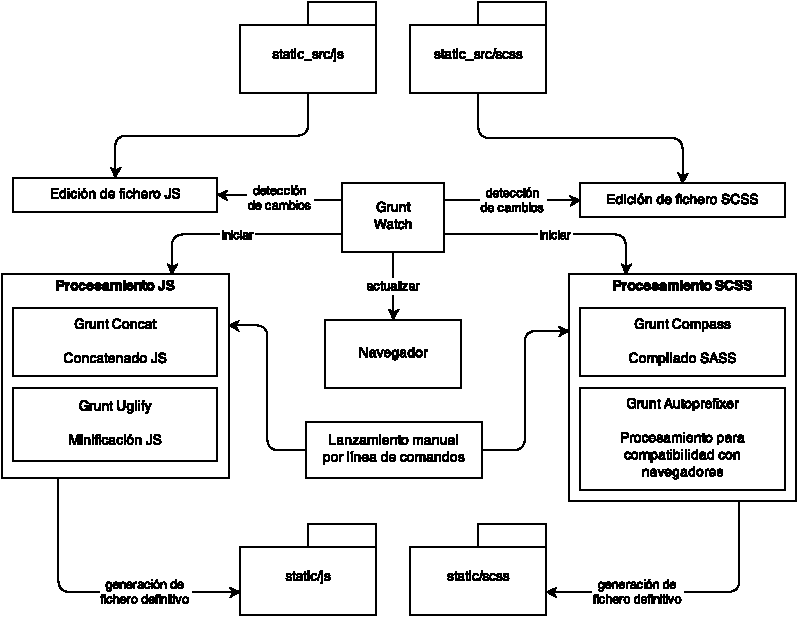
\includegraphics[width=\textwidth]{5_diseno/diagrama-frontend}
  \caption{Diagrama de flujo de trabajo del front-end}
  \label{fig:frontend}
\end{figure}

En la figura~\ref{fig:frontend} se puede ver una diagrama del flujo de
desarrollo de las hojas de estilo y del código JavaScript de la parte
frontend. El desarrollador trabaja dentro de la carpeta
\texttt{siteup\_frontend/static\_src}, que contiene los ficheros fuente de las
hojas de estilo y los scripts de JavaScript.

Se detallan a continuación los pasos que se siguen en el flujo de trabajo.

\subsubsection{Instalación de paquetes de desarrollo}

Para seguir este flujo de trabajo es necesario instalar ciertas dependencias en
el sistema. En particular, es necesario instalar el entorno node.js, según las
instrucciones de su distribución particular. Hecho esto, lo siguiente es
ejecutar el siguiente comando:

\begin{bashcode}
$ npm install  
\end{bashcode}

Esto generará un directorio \texttt{node\_modules} con las dependencias de node
instaladas. 

\subsubsection{Inicio del flujo de trabajo}

El siguiente paso es lanzar uno de los plugins de grunt,
\textbf{\texttt{grunt-contrib-watch}}, que se encarga de vigilar los cambios
sobre los ficheros. Cuando detecta cambios, hace dos cosas:

\begin{itemize}
\item Primero, lanza las tareas de procesamiento que se detallan a continuación.
\item Segundo, terminadas las tareas, lanza una señal para actualizar el
  navegador. Así se evita al usuario tener que ir al navegador y manualmente
  actualizar la web. Este proceso se conoce como \textbf{livereload}.
\end{itemize}

Este proceso se lanza utilizando el siguiente comando:

\begin{bashcode}
$ grunt watch
Running "watch" task
Waiting...
\end{bashcode}

También es posible lanzar el procesamiento de forma manual ejecutando el siguiente comando:

\begin{bashcode}
$ grunt  
\end{bashcode}

El primer paso del procesamiento es siempre \textbf{limpiar} los ficheros
generados previamente. Esta acción la lleva a cabo el plugin
\textbf{\texttt{grunt-contrib-clean}}.

\subsubsection{Procesamiento JS}

El procesamiento de los ficheros JavaScript consta de varios pasos. El primero
de ellos es la \textbf{concatenación} de todos los ficheros de código. Es una
buena práctica tener el menor número de ficheros anexos en una web para reducir
al mínimo el número de peticiones al servidor. Para esto se utiliza el plugin
\textbf{\texttt{grunt-contrib-concat}}, que navega por el directorio
\texttt{siteup\_frontend/static\_src/js} y concatena todos los ficheros
JavaScript que encuentre en un solo fichero.

El siguiente paso es la \textbf{minificación} del fichero generado. Básicamente
lo que se busca es reducir el tamaño final del fichero mediante varios procesos,
como la eliminación de espacios en blanco y la reducción de los nombres de las
variables. Esto lo lleva a cabo el plugin \textbf{\texttt{grunt-contrib-uglify}}

Hecho esto, se copia el fichero generado a la carpeta de salida
\texttt{siteup\_frontend/static/js}. Una muestra de la salida generada por Grunt
al realizar el procesamiento es la siguiente:

\begin{verbatim}
>> File "siteup_frontend/static_src/js/main.js" changed.

Running "clean:js" (clean) task
Cleaning siteup_frontend/static/js/main.js...OK

Running "concat:build" (concat) task
File "siteup_frontend/static/js/main.js" created.

Done, without errors.
Completed in 0.335s at Sat Apr 19 2014 19:00:22 GMT+0200 (CEST) - Waiting...
\end{verbatim}

\subsubsection{Procesamiento SCSS}

Como se mencionó previamente en la sección~\ref{sec:arquitectura-fisica},
para el desarrollo de las hojas de estilo se utilizó Sass, un superconjunto de
CSS que añade numerosas funcionalidades que habitualmente resultan tediosas de
hacer directamente en CSS. El único contra que tiene el uso de Sass es que los
ficheros no pueden ser interpretados directamente por los navegadores, sino que
es necesario compilarlos a CSS tradicional.

Así, el primer paso del procesamiento es la compilación de los ficheros
Sass. Esto lo lleva a cabo el plugin \textbf{\texttt{grunt-contrib-compass}},
que lee los ficheros situados en \texttt{siteup\_frontend/static\_src/scss} y
realiza la generación.

El siguiente paso es el procesamiento del fichero CSS generado para maximizar su
compatibilidad con todos los navegadores. Esto se hace leyendo las propiedades
CSS utilizadas y añadiendo prefijos en aquellos casos que sea necesario. El
plugin encargado de hacer este trabajo es
\textbf{\texttt{grunt-autoprefixer}}. Como ejemplo, si tenemos el siguiente
código original:

\begin{minted}{css}
a {
  transition: transform 1s
}
\end{minted}

Tras el procesamiento se convertirá a:

\begin{minted}{css}
a {
  -webkit-transition: -webkit-transform 1s;
  transition: -ms-transform 1s;
  transition: transform 1s
}
\end{minted}

Se ve que el plugin añade los prefijos necesarios para los navegadores basados
en WebKit y para Internet Explorer (\texttt{-webkit} y \texttt{-ms}
respectivamente).

Resulta interesante comentar que este plugin es configurable, de forma que
podamos decidir a qué navegadores vamos a dar soporte. Por defecto añade los
prefijos necesarios para soportar las dos últimas versiones de los navegadores
más populares.

Tras este proceso, el fichero generado se copia a la carpeta
\texttt{siteup\_frontend/static/css}.


%%% Local Variables: 
%%% mode: latex
%%% TeX-master: "../memoria"
%%% End: 
